\documentclass[titlepage,a4paper]{article}

\usepackage{a4wide}
\usepackage[colorlinks=true,linkcolor=black,urlcolor=blue,bookmarksopen=true]{hyperref}
\usepackage{bookmark}
\usepackage{fancyhdr}
\usepackage[spanish]{babel}
\usepackage[utf8]{inputenc}
\usepackage[T1]{fontenc}
\usepackage{graphicx}
\usepackage{float}

\pagestyle{fancy} % Encabezado y pie de página
\fancyhf{}
\fancyhead[L]{G\_02\_IS\_II }
\fancyhead[R]{Ingenería del Software II - UPM}
\renewcommand{\headrulewidth}{0.4pt}
\fancyfoot[C]{\thepage}
\renewcommand{\footrulewidth}{0.4pt}

\begin{document}
\begin{titlepage} % Carátula
	\hfill
\includegraphics[width=9cm]{logoupm.png}
    \centering
    \vfill
    \Huge \textbf{Ciclo 1 — Gestor de Torneos de Tenis}
    \vskip2cm
    \Large Ingenería del Software II\\
    Séptimo cuatrimestre 2024 
    \vfill
    \begin{tabular}{ | c | c | c | } % Datos del versionado
      \hline
      Identificación: & Modificación & Petición Cambio \\ \hline 
      ED\_V1\_G02: & Versión Inicial & PC 0 \\ \hline
      ED\_VX\_G02 & Por Rellenar & PC X \\ \hline
  	\end{tabular}
    \vfill
    \vfill
\end{titlepage}

\tableofcontents % Índice general
\newpage

\section{Introducción}\label{sec:intro} %revisar, texto de prueba
El presente informe reune el estandar para la documentación de los diferentes archivos que componen la solución del primer ciclo del trabajo práctico de la asignatura Ingenería del Software II, que consiste en la elaboración de un sistema de gestión de torneos de tenis. 

\section{Tipografía}\label{sec:tipo}

Utilizamos la tipografía estandar del editor de Overleaf, que se trata de Computer Modern, en tamaño normalsize para los textos contenidos en cada una de las secciones, que es el equivalente a tamaño 10. Para los títulos de las secciones se utiliza esta misma tipografía, pero en negrita, y en tamaño 14. 

\section{Uso de la plantilla}\label{sec:modelo}

Para el uso adecuado de esta plantilla, es necesario tener instalado el editor de Tex, o usar el editor online de Overleaf, rellenando los diferentes campos entre las secciones, manteniendo las especifaciones de formato dadas en el punto anterior.

\section{Figuras, tablas y fórmulas }\label{sec:diagramasdeclase}

A continuación se encuentra en forma de ejemplo el formato para la representación de figuras y tablas a lo largo del proyecto. Las imágenes deberán ser subidas a la misma carpeta de proyecto que el documento en que debe mostrarse.

\begin{figure}[H]
\centering
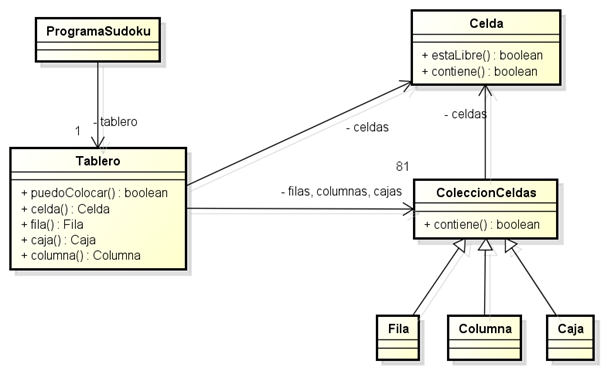
\includegraphics[width=0.8\textwidth]{diagrama_clase01.png}
\caption{\label{fig:class01} Ejemplo de Figura.}
\end{figure}

\begin{table}[h]
\centering
\begin{tabular}{ | c | c | c | }
    \hline
    Contenido 1 & Contenido 2 & Contenido 3 \\ \hline
    Ejemplo & Ejemplo & PC 0 \\ \hline
    Ejemplo & Ejemplo & PC X \\ \hline
\end{tabular}
\caption{Ejemplo de tabla}
\end{table}

\subsection{Fórmulas y Diagramas}
Para la representación de fórmulas se usarán diferentes funciones y librerías propias del editor, dependiendo de las necesidades del documento. En el caso de los diagramas, se realizan con herramientas externas, y se subirán los archivos para facilitar las modificaciones.



\end{document}
